
\subsection{Experiments with Deep Image Descriptors for Re-Identification}

% In this section we discuss the application of the described adaptation method to person re-identification \textit{(re-id}) problem.  The task of person re-identification is to associate people seen from different camera views. More formally, it can be defined as follows: given two sets of images from different cameras (\textit{probe} and \textit{gallery}) such that each person depicted in the probe set has an image in the gallery set,  for each image of a person from the probe set find an image of the same person in the gallery set.  Disjoint camera views, different illumination conditions, various poses and low quality of data make this problem difficult  even for humans (\eg, \citet{LiuLGW13} reports human performance at Rank1=$71.08\%$).  

% Unlike classification problems that are discussed above, re-identification problem implies that each image is mapped to a vector descriptor. The distance between descriptors is then used to match images from the probe set and the gallery set.
% To evaluate results of re-id methods the \textit{Cumulative Match Characteristic} (CMC) curve is commonly used. It is a plot of the identification rate (recall) at rank-$k$, that is the probability of the matching gallery image to be within the closest $k$ images (in terms of descriptor distance) to the probe image.

% Most existing works train descriptor mappings and evaluate them within the same data set containing images from a certain camera network with similar imaging conditions. Several papers, however, observed that the performance of the resulting re-identification systems drops very considerably when descriptors trained on one data set and tested on another. It is therefore natural to handle such cross-domain evaluation as a domain-adaptation problem, where each camera network (data set) constitutes a domain.

% Recently, several papers  with significantly improved re-identification performance \citep{ZhangS14a,ZhaoOW14,Paisitkriangkrai15} have been presented, with \citet{MaLYL15} reporting good results in cross-data-set evaluation scenario. At the moment, deep learning methods \citep{YiLL14} do not achieve state-of-the-art results probably because of the limited size of the training sets. Domain adaptation thus represents a viable direction for improving deep re-identification descriptors.

% \subsubsection{Data Sets and Protocols} 

% Following \citet{MaLYL15}, we use PRID \citep{Hirzer_h.:person}, VIPeR \citep{Gray07evaluatingappearance}, CUHK \citep{LiW13} as target data sets for our experiments.  

%------------------------to main intro------------
%The \textit{PRID} data set exists in two versions, and as in \citep{MaLYL15} we use a single-shot variant. It contains images of $385$ persons viewed from camera A and images of $749$ persons viewed from camera B,  $200$ persons appear in both cameras. The \textit{VIPeR} data set also contains images taken with two cameras, and in total $632$ persons are captured, for every person there is one image for each of the two camera views. The \textit{CUHK} data set consists of images from five pairs of cameras, two images for each person from each of the two cameras. We refer to the subset of this data set that includes the first pair of cameras only as \textit{CUHK/p1} (as most papers use this subset).

% We perform extensive experiments for various pairs of data sets, where one data set serves as a source domain, \ie, it is used to train a descriptor mapping in a supervised way with known correspondences between probe and gallery images. The second data set is used as a target domain, so that images from that data set are used without probe-gallery correspondence.

% In more detail, CUHK/p1 is used for experiments when CUHK serves as a target domain and two settings (``whole CUHK'' and CUHK/p1) are used for experiments when CUHK serves as a source domain. Given PRID as a target data set, we randomly choose 100 persons appearing in both camera views as training set. The images of the other 100 persons from camera A are used as probe, all images from camera B excluding those used in training (649 in total) are used as gallery at test time. For VIPeR, we use random 316 persons for training and all others for testing. For CUHK, 971 persons are split into 485 for training and 486 for testing.
% Unlike \citet{MaLYL15}, we use all images in the first  pair of cameras of CUHK instead of choosing one image of a person from each camera view. We also performed two experiments with all images of the whole CUHK data set as source domain and VIPeR and PRID data sets as target domains as in the  original paper \citep{YiLL14}.
------------------
\newlength\reidheight
\setlength{\reidheight}{2.5cm}

\addtolength{\tabcolsep}{-3pt}

\begin{figure*}
\centering
\begin{tabular}{cccc|cccc|cccc}
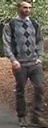
\includegraphics[height=\reidheight]{Chapters/gradrev/figures/dataset_samples/viper/a/000_45.png}&
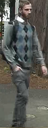
\includegraphics[height=\reidheight]{Chapters/gradrev/figures/dataset_samples/viper/b/000_45.png}&
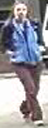
\includegraphics[height=\reidheight]{Chapters/gradrev/figures/dataset_samples/viper/a/001_45.png}&
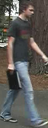
\includegraphics[height=\reidheight]{Chapters/gradrev/figures/dataset_samples/viper/b/002_90.png}&
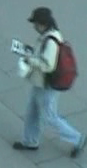
\includegraphics[height=\reidheight]{Chapters/gradrev/figures/dataset_samples/PRID/a/img_0001.png}&
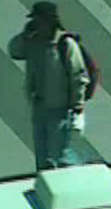
\includegraphics[height=\reidheight]{Chapters/gradrev/figures/dataset_samples/PRID/b/img_0001.png}&
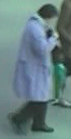
\includegraphics[height=\reidheight]{Chapters/gradrev/figures/dataset_samples/PRID/a/img_0002.png}&
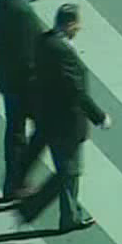
\includegraphics[height=\reidheight]{Chapters/gradrev/figures/dataset_samples/PRID/b/img_0003.png}&
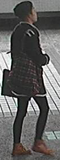
\includegraphics[height=\reidheight]{Chapters/gradrev/figures/dataset_samples/cuhk/a/001_00005.png}&
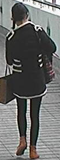
\includegraphics[height=\reidheight]{Chapters/gradrev/figures/dataset_samples/cuhk/b/001_00221.png}&
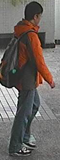
\includegraphics[height=\reidheight]{Chapters/gradrev/figures/dataset_samples/cuhk/a/002_00280.png}&
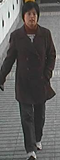
\includegraphics[height=\reidheight]{Chapters/gradrev/figures/dataset_samples/cuhk/b/003_00403.png}\\
\multicolumn{4}{c}{VIPER}&
\multicolumn{4}{c}{PRID}&
\multicolumn{4}{c}{CUHK}
\end{tabular}
\caption{Matching and non-matching pairs of probe-gallery images from different person re-identification data sets. The three data sets are treated as different domains in our experiments.}
\label{fig:reidsamples}
\end{figure*}

\addtolength{\tabcolsep}{3pt}

Following \citet{YiLL14}, we augmented our data with mirror images, and during test time we calculate similarity score between two images as the mean of the four scores corresponding to different flips of the two compared images. In case of CUHK, where there are 4 images (including mirror images) for each of the two camera views for each person, all 16 combinations' scores are averaged. 

\subsubsection{CNN architectures and Training Procedure} 

In our experiments, we use siamese architecture described in \citet{YiLL14} (\textit{Deep Metric Learning} or \textit{DML}) for learning deep image descriptors on the source data set.
This architecture incorporates two convolution layers (with $7\times7$ and $5\times5$ filter banks), followed by ReLU and max pooling, and one fully-connected layer, which gives $500$-dimensional descriptors as an output. There are three parallel flows within the CNN for processing three part of an image: the upper, the middle, and the lower one. The first convolution layer shares parameters between three parts, and the outputs of the second convolution layers are concatenated.
During training, we follow \citet{YiLL14} and calculate pairwise cosine similarities between $500$-dimensional features within each batch and backpropagate the loss for all pairs within batch. 

To perform domain-adversarial training, we construct a DANN architecture.  The feature extractor includes the two convolutional layers (followed by max-pooling and ReLU) discussed above. The label predictor in this case is replaced with \textit{descriptor predictor} that includes one fully-connected layer. The domain classifier includes two fully-connected layers with $500$ units in the intermediate representation ($x{\rightarrow}500{\rightarrow}1$). 

For the verification loss function in the descriptor predictor we used Binomial Deviance loss, defined in \citet{YiLL14} with similar parameters: $\alpha = 2$, $\beta = 0.5$, $c = 2$ (the asymmetric cost parameter for negative pairs). The domain classifier is trained with logistic loss as in subsection  \ref{train_proc_for_classification}.

We used learning rate fixed to $0.001$ and momentum of $0.9$. The schedule of adaptation similar to the one described in subsection \ref{train_proc_for_classification} was used. We also inserted dropout layer with rate $0.5$ after the concatenation of outputs of the second max-pooling layer. $128$-sized batches were used for source data and $128$-sized batches for target data. 

%TODO fix 
% \begin{figure*}[t]
%   \definecolor{fnodebottom}{RGB}{132,170,81}
%   \definecolor{fnodetop}{RGB}{172,222,106}
%   \definecolor{cnodebottom}{RGB}{120,128,164}
%   \definecolor{cnodetop}{RGB}{158,167,218}
%   \definecolor{dnodebottom}{RGB}{174,109,146}
%   \definecolor{dnodetop}{RGB}{230,141,192}
%   \centering
%   {%
%      \scalebox{0.65}{\input{./Chapters/gradrev/figures/archs/reidentification_adaptation.tikz}}}\\
%   \caption{CNN architecture used in experiments on domain adaptation for person re-identification}
%   \label{fig:reid_arch}
% \end{figure*}

\subsubsection{Results on Re-identification data sets} 

\begin{figure}[t]
\centering
  \begin{tabular}{p{5cm}  p{5cm}  p{5cm} }
      
        \setlength\figureheight{3.5cm}
        \setlength\figurewidth{3.5cm}
        \begin{tikzpicture}[font=\scriptsize]

\begin{axis}[%
width=0.95092\figurewidth,
height=\figureheight,
at={(0\figurewidth,0\figureheight)},
scale only axis,
xmin=1,
xmax=50,
xlabel={Rank},
ymin=0,
ymax=1,
ylabel={Identification rate (\%)},
axis x line*=bottom,
axis y line*=left,
legend style={at={($ (0,1) + (+0.1cm,+0.1cm) $)},anchor=north west,align=left,legend cell align=left,draw=black},
xmajorgrids,
ymajorgrids,
grid style={dashed}
]
\addplot [color=blue,solid,line width=1.0pt]
  table[row sep=crcr]{%
1    0.1518987341772152\\
5    0.34810126582278483\\
10   0.47468354430379744\\
15   0.5474683544303798\\
20   0.5886075949367089\\
25   0.629746835443038\\
30   0.6613924050632911\\
35   0.680379746835443\\
40   0.7120253164556962\\
45   0.7183544303797469\\
50   0.7310126582278481\\
};
\addlegendentry{DML};

\addplot [color=cyan,solid,line width=1.0pt]
  table[row sep=crcr]{%
1    0.14556962025316456\\
5    0.3322784810126582\\
10   0.4873417721518987\\
15   0.5569620253164557\\
20   0.5917721518987342\\
25   0.6424050632911392\\
30   0.689873417721519\\
35   0.7025316455696202\\
40   0.7278481012658228\\
45   0.7531645569620253\\
50   0.7848101265822784\\
};
\addlegendentry{DML, adaptation};



\end{axis}
\end{tikzpicture}%
        \centering\small{(a) Whole CUHK $\rightarrow$ VIPeR}
        \label{fig:allcuhk_viper}
  
    &
        \setlength\figureheight{3.5cm}
        \setlength\figurewidth{3.5cm}
        \begin{tikzpicture}[font=\scriptsize]

\begin{axis}[%
width=0.95092\figurewidth,
height=\figureheight,
at={(0\figurewidth,0\figureheight)},
scale only axis,
xmin=1,
xmax=50,
xlabel={Rank},
ymin=0,
ymax=1,
ylabel={Identification rate (\%)},
axis x line*=bottom,
axis y line*=left,
legend style={at={($ (0,1) + (+0.1cm,+0.1cm) $)},anchor=north west,align=left,legend cell align=left,draw=black},
xmajorgrids,
ymajorgrids,
grid style={dashed}
]
\addplot [color=blue,solid,line width=1.0pt]
  table[row sep=crcr]{%
1      0.126582278481 \\
5      0.303797468354 \\
10      0.414556962025 \\
15      0.490506329114 \\
20      0.550632911392 \\
25      0.613924050633 \\
30      0.651898734177 \\
35      0.686708860759 \\
40      0.708860759494 \\
45      0.75 \\
50      0.759493670886 \\
};
\addlegendentry{DML};

\addplot [color=cyan,solid,line width=1.0pt]
  table[row sep=crcr]{%
1      0.120253164557 \\
5      0.29746835443 \\
10      0.462025316456 \\
15      0.541139240506 \\
20      0.594936708861 \\
25      0.617088607595 \\
30      0.645569620253 \\
35      0.667721518987 \\
40      0.696202531646 \\
45      0.712025316456 \\
50      0.73417721519 \\
};
\addlegendentry{DML, adaptation};


\end{axis}
\end{tikzpicture}%
        \centering\small{(b) CUHK/p1 $\rightarrow$ VIPeR}
%        \label{fig:cuhk_p1_viper}
    &
        \setlength\figureheight{3.5cm}
        \setlength\figurewidth{3.5cm}
        \begin{tikzpicture}[font=\scriptsize]

\begin{axis}[%
width=0.95092\figurewidth,
height=\figureheight,
at={(0\figurewidth,0\figureheight)},
scale only axis,
xmin=1,
xmax=50,
xlabel={Rank},
ymin=0,
ymax=1,
ylabel={Identification rate (\%)},
axis x line*=bottom,
axis y line*=left,
legend style={at={($ (0,1) + (+0.1cm,+0.1cm) $)},anchor=north west,align=left,legend cell align=left,draw=black},
xmajorgrids,
ymajorgrids,
grid style={dashed}
]
\addplot [color=blue,solid,line width=1.0pt]
  table[row sep=crcr]{%
1      0.0664556962025 \\
5      0.167721518987 \\
10      0.253164556962 \\
15      0.275316455696 \\
20      0.316455696203 \\
25      0.348101265823 \\
30      0.379746835443 \\
35      0.414556962025 \\
40      0.45253164557 \\
45      0.474683544304 \\
50      0.496835443038 \\
};
\addlegendentry{DML};

\addplot [color=cyan,solid,line width=1.0pt]
  table[row sep=crcr]{%
1      0.0632911392405 \\
5      0.161392405063 \\
10      0.259493670886 \\
15      0.338607594937 \\
20      0.389240506329 \\
25      0.417721518987 \\
30      0.439873417722 \\
35      0.471518987342 \\
40      0.496835443038 \\
45      0.518987341772 \\
50      0.53164556962 \\
};
\addlegendentry{DML, adaptation};


\end{axis}
\end{tikzpicture}%
        \centering\small{(c) PRID $\rightarrow$ VIPeR}
%        \label{fig:cuhk_p1_viper} \\    
 \end{tabular}
%  \caption{Results on VIPeR}
%  \label{fig:viper}
% \end{figure}%

% \begin{figure}[h]
% \centering
 \begin{tabular}{ p{5cm}  p{5cm}  p{5cm} }
        \setlength\figureheight{3.5cm}
        \setlength\figurewidth{4cm}
        \begin{tikzpicture}[font=\scriptsize]

\begin{axis}[%
width=0.95092\figurewidth,
height=\figureheight,
at={(0\figurewidth,0\figureheight)},
scale only axis,
xmin=1,
xmax=50,
xlabel={Rank},
ymin=0,
ymax=1,
ylabel={Identification rate (\%)},
axis x line*=bottom,
axis y line*=left,
legend style={at={($ (0,1) + (+0.1cm,+0.1cm) $)},anchor=north west,align=left,legend cell align=left,draw=black},
xmajorgrids,
ymajorgrids,
grid style={dashed}
]
\addplot [color=blue,solid,line width=1.0pt]
  table[row sep=crcr]{%
1    0.08\\
5    0.13\\
10   0.22\\
15   0.27\\
20   0.31\\
25   0.35\\
30   0.4\\
35   0.41\\
40   0.41\\
45   0.43\\
50   0.44\\
};
\addlegendentry{DML};

\addplot [color=cyan,solid,line width=1.0pt]
  table[row sep=crcr]{%
1    0.07\\
5    0.19\\
10   0.27\\
15   0.32\\
20   0.35\\
25   0.37\\
30   0.39\\
35   0.41\\
40   0.43\\
45   0.45\\
50   0.45\\
};
\addlegendentry{DML, adaptation};


%[0.08, 0.13, 0.22, 0.27, 0.31, 0.35, 0.4, 0.41, 0.41, 0.43, 0.44]
%[0.07, 0.19, 0.27, 0.32, 0.35, 0.37, 0.39, 0.41, 0.43, 0.45, 0.45]

%
\end{axis}
\end{tikzpicture}%





        \centering\small{(d) Whole CUHK $\rightarrow$ PRID}
        \label{fig:allcuhk_prid}
    &
        \setlength\figureheight{3.5cm}
        \setlength\figurewidth{4cm}
        \begin{tikzpicture}[font=\scriptsize]

\begin{axis}[%
width=0.95092\figurewidth,
height=\figureheight,
at={(0\figurewidth,0\figureheight)},
scale only axis,
xmin=1,
xmax=50,
xlabel={Rank},
ymin=0,
ymax=1,
ylabel={Identification rate (\%)},
axis x line*=bottom,
axis y line*=left,
legend style={at={($ (0,1) + (+0.1cm,+0.1cm) $)},anchor=north west,align=left,legend cell align=left,draw=black},
xmajorgrids,
ymajorgrids,
grid style={dashed}
]
\addplot [color=blue,solid,line width=1.0pt]
  table[row sep=crcr]{%
1      0.04 \\
5      0.08 \\
10      0.15 \\
15      0.22 \\
20      0.25 \\
25      0.3 \\
30      0.32 \\
35      0.36 \\
40      0.39 \\
45      0.41 \\
50      0.44 \\
};
\addlegendentry{DML};

\addplot [color=cyan,solid,line width=1.0pt]
  table[row sep=crcr]{%
1      0.06 \\
5      0.16 \\
10      0.21 \\
15      0.27 \\
20      0.31 \\
25      0.36 \\
30      0.39 \\
35      0.41 \\
40      0.41 \\
45      0.42 \\
50      0.43 \\
};
\addlegendentry{DML, adaptation};


\end{axis}
\end{tikzpicture}%
        \centering\small{(e) CUHK/p1 $\rightarrow$ PRID}
        \label{fig:cuhk_p1_prid}
    &
       \setlength\figureheight{3.5cm}
       \setlength\figurewidth{4cm}
       \begin{tikzpicture}[font=\scriptsize]

\begin{axis}[%
width=0.95092\figurewidth,
height=\figureheight,
at={(0\figurewidth,0\figureheight)},
scale only axis,
xmin=1,
xmax=50,
xlabel={Rank},
ymin=0,
ymax=1,
ylabel={Identification rate (\%)},
axis x line*=bottom,
axis y line*=left,
legend style={at={($ (0,1) + (+0.1cm,+0.1cm) $)},anchor=north west,align=left,legend cell align=left,draw=black},
xmajorgrids,
ymajorgrids,
grid style={dashed}
]
\addplot [color=blue,solid,line width=1.0pt]
  table[row sep=crcr]{%
1      0.08 \\
5      0.15 \\
10      0.19 \\
15      0.25 \\
20      0.28 \\
25      0.34 \\
30      0.35 \\
35      0.36 \\
40      0.39 \\
45      0.4 \\
50      0.41 \\
};
\addlegendentry{DML};

\addplot [color=cyan,solid,line width=1.0pt]
  table[row sep=crcr]{%
1      0.07 \\
5      0.19 \\
10      0.25 \\
15      0.27 \\
20      0.31 \\
25      0.36 \\
30      0.39 \\
35      0.42 \\
40      0.42 \\
45      0.46 \\
50      0.47 \\
};
\addlegendentry{DML, adaptation};


\end{axis}
\end{tikzpicture}%
        \centering\small{(f) VIPeR $\rightarrow$ PRID}
        \label{fig:viper_prid}  \\    
 \end{tabular}
%  \caption{Results on PRID}
%  \label{fig:prid}
% \end{figure}


% \begin{figure}[h]
% \centering
 \begin{tabular}{ p{5cm}  p{5cm}}
        \setlength\figureheight{3.5cm}
        \setlength\figurewidth{4cm}
        \begin{tikzpicture}[font=\scriptsize]

\begin{axis}[%
width=0.95092\figurewidth,
height=\figureheight,
at={(0\figurewidth,0\figureheight)},
scale only axis,
xmin=1,
xmax=50,
xlabel={Rank},
ymin=0,
ymax=1,
ylabel={Identification rate (\%)},
axis x line*=bottom,
axis y line*=left,
legend style={at={($ (0,1) + (+0.1cm,+0.1cm) $)},anchor=north west,align=left,legend cell align=left,draw=black},
xmajorgrids,
ymajorgrids,
grid style={dashed}
]
\addplot [color=blue,solid,line width=1.0pt]
  table[row sep=crcr]{%
1      0.109053497942 \\
5      0.265432098765 \\
10      0.366255144033 \\
15      0.407407407407 \\
20      0.465020576132 \\
25      0.491769547325 \\
30      0.510288065844 \\
35      0.541152263374 \\
40      0.572016460905 \\
45      0.59670781893 \\
50      0.617283950617 \\
};
\addlegendentry{DML};

\addplot [color=cyan,solid,line width=1.0pt]
  table[row sep=crcr]{%
1      0.125514403292 \\
5      0.253086419753 \\
10      0.366255144033 \\
15      0.440329218107 \\
20      0.5 \\
25      0.5329218107 \\
30      0.572016460905 \\
35      0.594650205761 \\
40      0.617283950617 \\
45      0.650205761317 \\
50      0.668724279835 \\
};
\addlegendentry{DML, adaptation};


\end{axis}
\end{tikzpicture}%
        \centering\small{(g) VIPeR $\rightarrow$ CUHK/p1}
        \label{fig:viper_cuhk_p1}
    &
        \setlength\figureheight{3.5cm}
        \setlength\figurewidth{4cm}
        \begin{tikzpicture}[font=\scriptsize]

\begin{axis}[%
width=0.95092\figurewidth,
height=\figureheight,
at={(0\figurewidth,0\figureheight)},
scale only axis,
xmin=1,
xmax=50,
xlabel={Rank},
ymin=0,
ymax=1,
ylabel={Identification rate (\%)},
axis x line*=bottom,
axis y line*=left,
legend style={at={($ (0,1) + (+0.1cm,+0.1cm) $)},anchor=north west,align=left,legend cell align=left,draw=black},
xmajorgrids,
ymajorgrids,
grid style={dashed}
]
\addplot [color=blue,solid,line width=1.0pt]
  table[row sep=crcr]{%
1      0.0569620253165 \\
5      0.139240506329 \\
10      0.212025316456 \\
15      0.284810126582 \\
20      0.316455696203 \\
25      0.344936708861 \\
30      0.370253164557 \\
35      0.389240506329 \\
40      0.414556962025 \\
45      0.443037974684 \\
50      0.465189873418 \\
};
\addlegendentry{DML};

\addplot [color=cyan,solid,line width=1.0pt]
  table[row sep=crcr]{%
1      0.0843621399177 \\
5      0.191358024691 \\
10      0.263374485597 \\
15      0.316872427984 \\
20      0.347736625514 \\
25      0.395061728395 \\
30      0.432098765432 \\
35      0.471193415638 \\
40      0.504115226337 \\
45      0.5329218107 \\
50      0.553497942387 \\
};
\addlegendentry{DML, adaptation};


\end{axis}
\end{tikzpicture}%
        \centering\small{(h) PRID $\rightarrow$ CUHK/p1}
        \label{fig:prid_cuhk_p1}
  \\    
  \end{tabular}
  \caption{Results on VIPeR, PRID and CUHK/p1 with and without domain-adversarial learning. Across the eight domain pairs domain-adversarial learning improves re-identification accuracy. For some domain pairs the improvement is considerable.}
  \label{fig:adaptresults}
\end{figure}

Figure \ref{fig:adaptresults} shows results in the form of CMC-curves for eight pairs of data sets. Depending on the hardness of the annotation problem we trained either for 50,000 iterations (CUHK/p1 $\rightarrow$ VIPeR, VIPeR $\rightarrow$ CUHK/p1, PRID $\rightarrow$ VIPeR) or for 20,000 iterations (the other five pairs). 

\begin{figure*}
\centering
\begin{tabular}{c c}
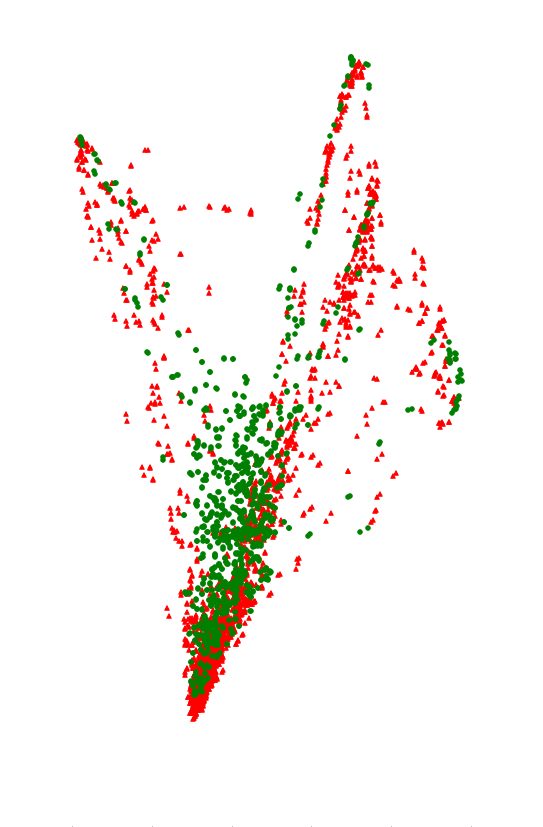
\includegraphics[height=7cm, width=7cm]{./Chapters/gradrev/figures/reid_adapt_results/viper_cuhkp1_zc.png}&
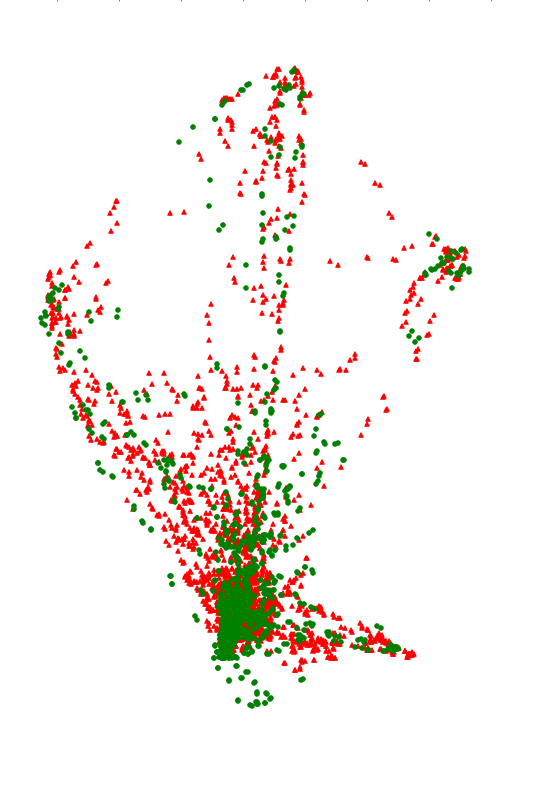
\includegraphics[height=7cm, width=7cm]{./Chapters/gradrev/figures/reid_adapt_results/viper_cuhkp1_da.png}\\
\small{(a) DML}&
\small{(b) DML, adaptation}\\
\end{tabular}
\caption{The effect of adaptation shown by t-SNE visualizations of source and target domains descriptors in a VIPeR $\rightarrow$ CUHK/p1 experiment pair. VIPeR is depicted with \textit{green} and CUHK/p1 - with \textit{red}. As in the image classification case, domain-adversarial learning ensures a closer match between the source and the target distributions. }
\label{fig:reidtsne}
\end{figure*}


After the sufficient number of iterations, domain-adversarial training consistently improves the performance of re-identification. For the pairs that involve PRID data set, which is more dissimilar to the other two data sets, the improvement is considerable. Overall, this demonstrates the applicability of the domain-adversarial learning beyond classification problems.

Figure \ref{fig:reidtsne} further demonstrates the effect of adaptation on the distributions of the learned descriptors in the source and in target sets in VIPeR $\rightarrow$ CUHK/p1 experiments, where domain adversarial learning once again achieves better intermixing of the two domains.


\section{Conclusion}

The paper proposes a new approach to domain adaptation of feed-forward neural networks, which allows large-scale training based on large amount of annotated data in the source domain and large amount of unannotated data in the target domain. Similarly to many previous shallow and deep DA techniques, the adaptation is achieved through aligning the distributions of features across the two domains. However, unlike previous approaches, the alignment is accomplished through standard backpropagation training.

The approach is motivated and supported by the domain adaptation theory of \citet{BenDavid-NIPS06,BenDavid-MLJ2010}. 
The main idea behind DANN is to enjoin the network hidden layer to learn a representation which is predictive of the source example labels, but uninformative about the domain of the input (source or target). 
We implement this new approach within both shallow and deep feed-forward architectures. The latter allows simple implementation within virtually any deep learning package through the introduction of a simple gradient reversal layer. 
We have shown that our approach is flexible and achieves state-of-the-art results on a variety of benchmark in domain adaptation, namely for sentiment analysis and image classification tasks. 

A convenient aspect of our approach is that the domain adaptation component can be added to almost any neural network architecture that is trainable with backpropagation. Towards this end, We have demonstrated experimentally that the approach is not confined to classification tasks but can be used in other feed-forward architectures, e.g.\ for descriptor learning for person re-identification.